\documentclass[12pt,answers]{exam}
\usepackage[utf8]{inputenc}
\usepackage{notomath, noto-mono}
\usepackage{siunitx}
\usepackage{amsmath}

\usepackage{pgfplots}
\pgfplotsset{compat=1.9}
\usepgfplotslibrary{external}
\tikzexternalize

\title{Revision Exercise}
\author{T2W10 HBL}
\date{25 May 2022}

\newcommand{\cm}{\si{\centi\metre} }

\begin{document}
\maketitle

\begin{questions}

\question The figure below shows two right-angled triangles.
Given that \(PQ = x\) \cm, \(PR = (x + 8)\) \cm, \(QR = (x + 4)\) \cm,
and \(SQ = 5\) \cm, find the length of \(PS\).

\begin{figure}[htpb]
	\centering
	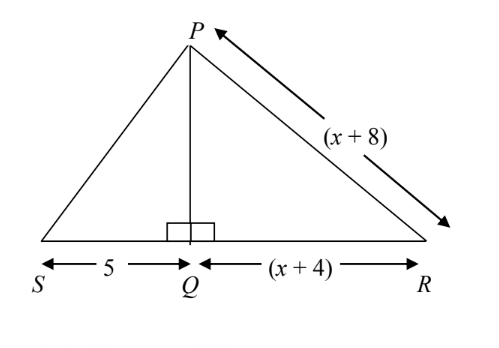
\includegraphics{tri.png}
	\caption{Two right-angled triangles.}
	\label{fig:tri}
\end{figure}

\begin{solution}
\begin{align*}
	x^2 + (x + 4)^2 &= (x + 8)^2 \\
	2x^2 + 8x + 16 &= x^2 + 16x + 64 \\
	x^2 - 8x - 48 &= 0 \\
	(x + 4)(x - 12) &= 0 \\
	x &= -4 \text{ (rej.) or } 12 \\
	\therefore PS &= \sqrt{x^2 + 5^2} \\
	&= \sqrt{12^2 + 5^2} \\
	&= 13
\end{align*}
The length of \(PS\) is 13 \cm.
\end{solution}

\question The diagram shows part of the graph \(y = 20 + 3x - 2x^2\).
The graph cuts the axis at \(P\) and \(R\) and the \(y\)-axis at \(Q\).
\begin{figure}[htpb]
	\centering
	\begin{tikzpicture}
	\begin{axis}[axis lines=center,xtick=\empty, ytick=\empty,ymin=-10,ymax=25]
	\addplot[color=black, domain=-5:10,smooth]{20+3*x-2*x^2};
	\addplot[draw=none,black,mark=*,nodes near coords={\(Q\)}] coordinates {(0, 20)};
	\addplot[draw=none,black,mark=*,nodes near coords={\(P\)}] coordinates {(-2.5,0)};
	\addplot[draw=none,black,mark=*,nodes near coords={\(R\)}] coordinates {(4, 0)};
	\end{axis}
	\end{tikzpicture}
	\caption{The graph of \(y = 20 + 3x - 2x^2\).}
	\label{fig:grph}
\end{figure}
\begin{parts}
\part Find the coordinates of $P$, $Q$ and $R$.
\begin{solution}
\begin{align*}
	Q &= (0, 20) \\
	y &= 20 + 3x - 2x^2 \\
	&= -(2x + 5)(x - 4) \\
	-(2x + 5)(x - 4) &= 0 \\
	x &= -\dfrac{5}{2} \text{ or } 4 \\
	\therefore P &= \left(-\dfrac{5}{2}, 0\right) \\
	\therefore R &= \left(4, 0\right)
\end{align*}
\end{solution}

\part Write down the equation of the line of symmetry of the graph \(y = 20 + 3x - 2x^2\).
\begin{solution}
\begin{align*}
		x &= \dfrac{-\dfrac{5}{2} + 4}{2} \\ 
		&= \dfrac{3}{4}
\end{align*}
\end{solution}
\end{parts}

\question In the diagram, \(AC = 26\) \cm, \(BD = 7\) \cm, \(BC = 10\) \cm,
and \(\angle ABC =\) \ang{90}. Calculate
\begin{figure}
	\centering
	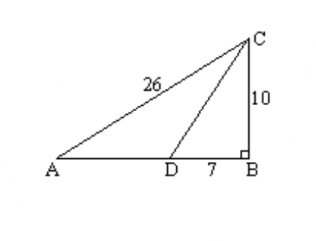
\includegraphics{tri2.png}
	\caption{Question 3.}
	\label{fig:trings}
\end{figure}
\begin{parts}
\part \(AD\),
\begin{solution}
\begin{align*}
		AD &= \sqrt{26^2 - 10^2} - 7 \\
		&= 17 \text{ \cm}
\end{align*}
\end{solution}
\part the area of \(\Delta ACD\).
\begin{solution}
\begin{align*}
	\Delta ACD &= \dfrac{17 \times 10}{2} \\
	&= 85 \text{ \si{\square\centi\metre}}
\end{align*}
\end{solution}
\end{parts}

\question \(VABCD\) is a pyramid with a square base $ABCD$ and a height $VN$. Given that the height, $VN$, is 12 \cm and the volume of the pyramid is 400 \si{\cubic\centi\metre}, calculate the
\begin{figure}[htpb]
	\centering
	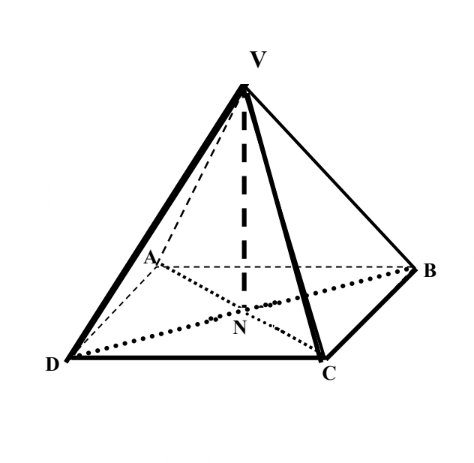
\includegraphics[scale=0.5]{pyt.png}
	\caption{Pyramid \(VABCD\).}
	\label{fig:pyr}
\end{figure}
\begin{parts}
\part length of the side of the square base,
\begin{solution}
\begin{align*}
	\text{length of the side of the square base } &= \sqrt{\dfrac{400 \div \dfrac{1}{3}}{12}} \\
	&= 10 \text{ \cm}
\end{align*}
\end{solution}
\part total surface area of the pyramid.
\begin{solution}
\begin{align*}
	\text{total surface area } &= 10^2 + 4 \times \dfrac{1}{2} \times 10 \times \sqrt{\left(\dfrac{10}{2}\right)^2 + 12^2} \\
	&= 100 + 2 \times 130 \\
	&= 360 \text{ \si{\square\centi\metre}}
\end{align*}
\end{solution}
\end{parts}

\question In the given diagram, \(AD = 16\) \cm, $BD = 10$ \cm, and $CD = 8$ \cm. \(M\) lies on the line $AD$. Find
\begin{figure}
	\centering
	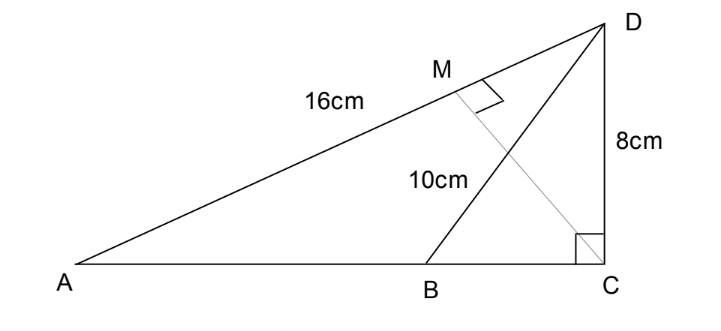
\includegraphics[scale=.7]{tri3.png}
	\caption{Question 5.}
	\label{fig:abj}
\end{figure}
\begin{parts}
\part $BC$.
\begin{solution}
\begin{align*}
	BC &= \sqrt{10^2 - 8^2} \\
	&= 6 \text{ \cm}
\end{align*}
\end{solution}

\part $AB$.
\begin{solution}
\begin{align*}
	AB &= \sqrt{16^2 - 8^2} - 6 \\
	&= \left(8\sqrt{3} - 6\right) \text{ \cm} \\
	&= 7.86 \text{ \cm\,(3 s.f.)}
\end{align*}
\end{solution}

\part the area of $\Delta ACD$.
\begin{solution}
\begin{align*}
	\text{area of } \Delta ACD &= 8\sqrt{3} \times 8 \times \dfrac{1}{2} \\
	&= 32\sqrt{3} \text{ \si{\square\centi\metre}} \\
	&= 55.4 \text{ \si{\square\centi\metre} (3 s.f.)}
\end{align*}
\end{solution}
\part $CM$.
\begin{solution}
\begin{align*}
	\text{area of } \Delta ACD &= \dfrac{1}{2} \times CM \times 16 \\
	CM &= 32\sqrt{3} \div 8 \\
	&= 4\sqrt{3} \\
	&= 6.93 \text{\cm  (3 s.f.)}
\end{align*}

The length of $CM$ is 6.93 \cm  (3 s.f.).
\end{solution}
\end{parts}

\question Simplify the expressions, expressing your answer in positive indices.
\begin{parts}
\part $g^3\left(\dfrac{h^2}{g^4}\right)^2 \div \left(\dfrac{g^{-2}h^3}{g^2h}\right)^{-3}$
\begin{solution}
\begin{align*}
	g^3\left(\dfrac{h^2}{g^4}\right)^2 \div \left(\dfrac{g^{-2}h^3}{g^2h}\right)^{-3} &= g^3\left(\dfrac{h^4}{g^8}\right) \div \left(\dfrac{h^2}{g^4}\right)^{-3} \\
	&= \dfrac{g^3h^4}{g^8} \times \left(\dfrac{h^2}{g^4}\right)^3 \\
	&= \dfrac{h^4}{g^5} \times \dfrac{h^6}{g^{12}} \\
	&= \dfrac{h^{10}}{g^{17}}
\end{align*}
\end{solution}

\part $\left(-\dfrac{4}{5}xy^3\right)^2 \times \left(-2x^2y\right)^{-3}$
\begin{solution}
\begin{align*}
	\left(-\dfrac{4}{5}xy^3\right)^2 \times \left(-2x^2y\right)^{-3} &= \dfrac{16}{25}x^2y^6 \cdot \dfrac{1}{\left(-2x^2y\right)^3} \\
	&= \dfrac{\dfrac{16}{25}x^2y^6}{-8x^6y^3} \\
	&= -\dfrac{2y^3}{25x^4}
\end{align*}
\end{solution}

\part $\left(16a^4\right)^\frac{1}{4} \times \left(\dfrac{1}{1000a^3}\right)^\frac{1}{3}$
\begin{solution}
\begin{align*}
	\left(16a^4\right)^\frac{1}{4} \times \left(\dfrac{1}{1000a^3}\right)^\frac{1}{3} &= \left(2^4 \cdot a^4\right)^\frac{1}{4}  \cdot \left(\dfrac{1}{10^3 \cdot a^3}\right)^\frac{1}{3} \\
	&= 2a \cdot \dfrac{1}{10a} \\
	&= \dfrac{1}{5}
\end{align*}
\end{solution}

\part $\left(m^3 \times m^{-4}\right)^{-2} + 2m^\frac{1}{2} \times m^\frac{1}{4} \times m^{1\frac{1}{4}}$
\begin{solution}
\begin{align*}
	\left(m^3 \times m^{-4}\right)^{-2} + 2m^\frac{1}{2} \times m^\frac{1}{4} \times m^{1\frac{1}{4}}
	&= \left(\dfrac{1}{m}\right)^{-2} + 2m^2 \\
	&= m^2 + 2m^2 \\
	&= 3m^2
\end{align*}
\end{solution}
\end{parts}

\question Rectangle $ABCD$ has length $AB = (5 - 2x)$ \cm, and breadth $BC = (7 - x)$ \cm.
\begin{figure}
		\centering
		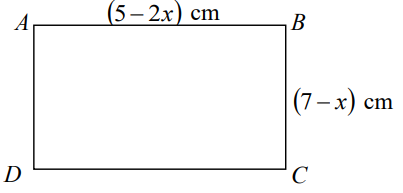
\includegraphics{rec.png}
		\caption{Rectangle $ABCD$.}
		\label{fig:rec}
\end{figure}

\begin{parts}
\part Write down an expression for the perimeter of the rectangle,
leaving your answer in terms of $x$. \label{7i}
\begin{solution}
\begin{align*}
		\text{perimeter of rect. } &= 2\left[(5 - 2x) + (7 - x)\right] \\
		&= 2(-3x + 12) \\
		&= (-6x + 24) \text{ \cm}
\end{align*}
\end{solution}

\part Given that the rectangle has an area of \qty{110}{\square\centi\metre},
write down an equation in $x$ and show that it reduces to $2x^2 - 19x - 75 = 0$.
\begin{solution}
\begin{align*}
		(5 - 2x)(7 - x) &= 110 \\
		35 - 14x - 5x + 2x^2 &= 110 \\
		2x^2 - 19x + 35 &= 110 \\
		2x^2 - 19x - 75 &= 0 
\end{align*}
\end{solution}

\part Expand $(2x - 25)(x + 3)$.
\begin{solution}
\begin{align*}
		(2x - 25)(x + 3) &= 2x^2 - 25x + 6x - 75 \\
		&= 2x^2 + 19x - 75
\end{align*}
\end{solution}

\part Solve the equation $2x^2 + 19x - 75 = 0$.
\begin{solution}
\begin{align*}
		2x^2 + 19x - 75 &= 0 \\
		(2x - 25)(x + 3) &= 0 \\
		x &= \dfrac{25}{2} \text{ or } -3
\end{align*}
\end{solution}

\part Substitute both values of $x$ into your expression in \textbf{(\ref{7i})}
and explain why you need to reject one of the values.
\begin{solution}

Case 1:
\begin{align*}
	-6x + 24 &= -6 \times \dfrac{25}{2} + 24 \\
	&= -51 \text{ \bf(rej.)}
\end{align*}

Case 2:
\begin{align*}
	-6x + 24 &= -6 \times (-3) + 24 \\
	&= 42
\end{align*}

The solution of $x = \dfrac{25}{2}$ needs to be rejected as it yields
a negative result when substituted into the expression for the rectangle's
perimeter, since a rectangle's perimeter cannot be of negative length.
\end{solution}
\end{parts}

\question Solve for $x$ in the following equations.
\begin{parts}
\part $2^x \div 4^{x - 3} \times 8^{3x + 1} = 0.25$.
\begin{solution}
\begin{align*}
	2^x \div 4^{x - 3} \times 8^{3x + 1} &= 0.25 \\
	2^x \div 2^{2x - 6} \times 2^{9x + 3} &= 2^{-2} \\
	x - (2x - 6) + (9x + 3) &= -2 \\
	8x + 9 &= -2 \\
	x &= -\dfrac{11}{8}
\end{align*}
\end{solution}

\part $8^{-2} \times 2^{2x} = \sqrt{4^{3x + 5}}$.
\begin{solution}
\begin{align*}
	8^{-2} \times 2^{2x} &= \sqrt{4^{3x + 5}} \\
	2^{2x - 6} &= 2^{3x + 5} \\
	2x - 6 &= 3x + 5 \\
	x + 5 &= -6 \\
	x &= -11
\end{align*}
\end{solution}

\part $2 \times 9^{2000} + 9^{2000} = 3^x$
\begin{solution}
\begin{align*}
	2 \times 9^{2000} + 9^{2000} &= 3^x \\
	3^1 \times 3^{4000} &= 3^x \\
	x &= 4001
\end{align*}
\end{solution}

\part $8^{3x + 2} = 0.03125$
\begin{solution}
\begin{align*}
	8^{3x + 2} &= 0.03125 \\
	2^{9x + 6} &= 2^{-5} \\
	9x + 6 &= -5 \\
	x &= -\dfrac{11}{9}
\end{align*}
\end{solution}

\part $2^{2008} + 2^{2008} + 2^{2008} + 2^{2008} + 2^{2008} + 2^{2008} + 2^{2008} + 2^{2008} = 2^x$
\begin{solution}
\begin{align*}
	2^{2008} + 2^{2008} + 2^{2008} + 2^{2008} + 2^{2008} + 2^{2008} + 2^{2008} + 2^{2008} &= 2^x \\
	2^3 \times 2^{2008} &= 2^x \\
	x &= 2011
\end{align*}
\end{solution}

\part $8^{3x + 2} = \dfrac{2^x}{32}$
\begin{solution}
\begin{align*}
	8^{3x + 2} &= \dfrac{2^x}{32} \\
	2^{9x + 6} &= 2^{x - 5} \\
	9x + 6 &= x - 5 \\
	x &= -\dfrac{11}{8}
\end{align*}
\end{solution}

\part $81^{3x - 7} = 243^x \div 27^{x - 4}$
\begin{solution}
\begin{align*}
	81^{3x - 7} &= 243^x \div 27^{x - 4} \\
	3^{12x - 28} &= 3^{5x} \div 3^{3x - 12} \\
	12x - 28 &= 2x + 12 \\
	10x &= 40 \\
	x &= 4
\end{align*}
\end{solution}
\end{parts}

\question Given that \(p = \) \num{4e2} and \(q = \) \num{2e-4}, evaluate, leaving your answer in standard form,
\begin{parts}
\part \(\dfrac{1}{q} + 2p\),
\begin{solution}
\begin{align*}
	\dfrac{1}{q} + 2p &= \dfrac{1}{\num{2e-4}} + \num{8e2} \\
	&= \dfrac{1}{2} \times 10^4 + \num{8e2} \\
	&= \num{5e3} + \num{8e2} \\
	&= \num{5.8e3}
\end{align*}
\end{solution}

\part \(\dfrac{p}{q}\)
\begin{solution}
\begin{align*}
	\dfrac{p}{q} &= \dfrac{\num{4e2}}{\num{2e-4}} \\
	&= \num{2e6}
\end{align*}
\end{solution}
\end{parts}

\question
\begin{parts}
\part Express \qty{2.05}{\centi\metre} in \si{\kilo\metre}, giving your answer in standard form.
\begin{solution}
$\qty{2.05}{\centi\metre} = \qty{2.05e-5}{\kilo\metre}$
\end{solution}

\part Evaluate $\num{2.4e-3} - \num{7.8e-2}$, giving your answer in standard form.
\begin{solution}
\begin{align*}
	\num{2.4e-3} - \num{7.8e-2} &= \num{0.24e-2} - \num{7.8e-2} \\
	&= \num{-7.56e-2}
\end{align*}
\end{solution}
\end{parts}

\question Identify the errors in the solution given below by rewriting the correct solution,
and showing all the necessary workings.

\textit{Evaluate the expression $\num{5.86e-2}-\num{9.2e-3}$, giving your answer in standard form.}
\begin{align*}
	\num{5.86e-2}-\num{9.2e-3} &= (5.86-9.2\times10)\times10^{-2} \\
	&= (5.86-92)\times10^{-2} \\
	&= \num{-86.14e-2}
\end{align*}

\begin{solution}
\begin{align*}
	\num{5.86e-2}-\num{9.2e-3} &= (5.86 - 9.2 \div 10) \times 10^{-2} \\
	&= (5.86 - 0.92) \times 10^{-2} \\
	&= \num{4.94e-2}
\end{align*}
\end{solution}
\end{questions}
\end{document}
